\documentclass[12pt]{report}

\usepackage[english]{babel}
\usepackage[utf8x]{inputenc}
\usepackage{amsmath}
\usepackage{graphicx}
\usepackage{multirow}
\usepackage[hypcap]{caption}
\usepackage{setspace} 
\usepackage{float}

\title{Lab 3: Strengthening Mechanisms and Aluminum Alloys}
\author{Zachary Tschirhart \\
	\small \\
        \small EID: zst75 \\
	\small Department of Aerospace Engineering and Engineering Mechanics \\
	\small \textbf{ASE 324L (Mon 2:00-5:00)} \\
	\small Unique: 13740}

\date{February 10, 2014}


\begin{document}
\maketitle

\begin{abstract}

\end{abstract}


\tableofcontents
\pagebreak

\setcounter{secnumdepth}{0}



\section{Introduction}
\doublespacing



\section{Experimental and Data Reduction Procedures}


\begin{equation}
        \sigma = \frac{4P}{\pi d_0^2}
	\label{equation:equation1}
\end{equation}


\section{Results and Discussion}
\doublespacing

%\begin{figure}[H]
%	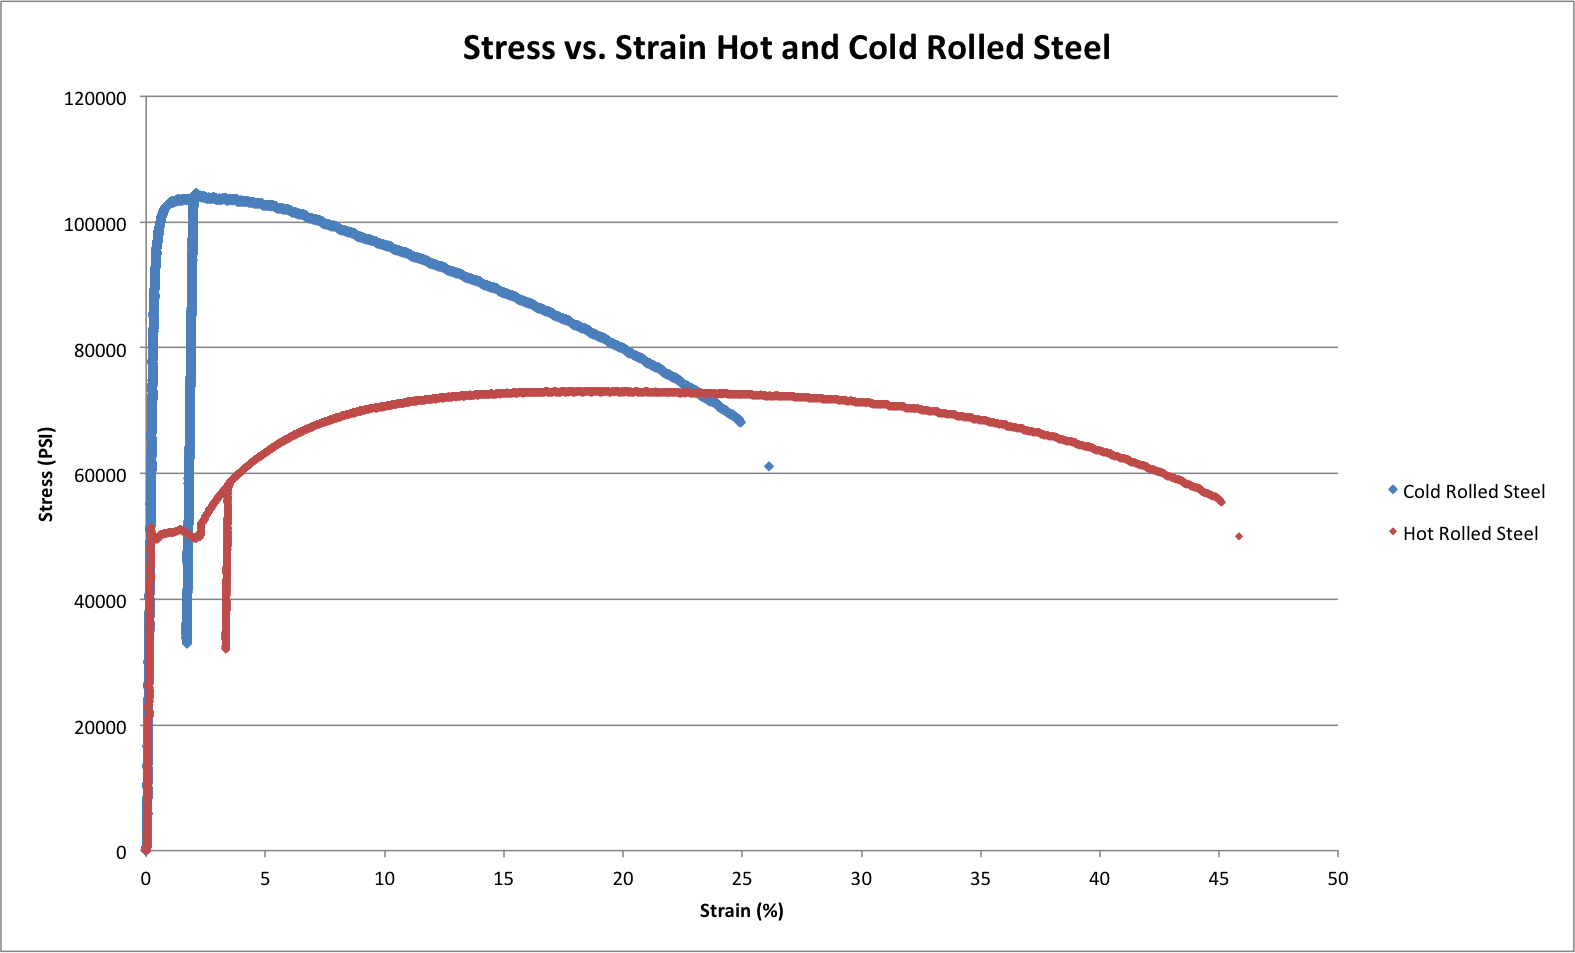
\includegraphics[width=1\textwidth]{stress_vs_strain.png}
%	\caption{Engineering stress vs. strain for Hot Rolled Steel}
%	\label{fig:Figure1}
%\end{figure}

\section{Conclusion}
\doublespacing



\begin{thebibliography}{0}
\bibitem{notes} {\em ASE 324L Lab manual : The University of Texas at Austin Department of Aerospace Engineering}  2014.
\bibitem{notes} {\em ASE 324L Lecture 5 : The University of Texas at Austin Department of Aerospace Engineering}  2014.
\end{thebibliography}
\addcontentsline{toc}{section}{Bibliography}


\end{document}
